\section{Automata Theory}
In this paper, we strictly observe probabilistic timed automata and refer to them as \textit{observed systems}.
%
Therefore, we begin this section by first explaining how time is handled in timed automata, followed by the formal definition of a timed automaton, and at the end we extend the definition to describe a probabilistic timed automaton.

\subsection{Time}
Time in timed automata is managed by units of \textit{clocks}, along with \textit{constraints} and \textit{interpretations} that represent the duration of a simulation of an automaton from the beginning until the end. We review the formal definition of the previous terms and also the definition of \textit{zones} in timed automata, as the terms will be used in the next sections. 
%
\theoremstyle{definition}
\begin{definition}{(Clock constraints and clock interpretations)} \cite{timedAutomata}
	For a set $X$ of clocks, the set $\Phi (X)$ of \textit{clock constraints} $\varphi$ is defined by the grammar 
	\begin{equation}
		\varphi := x \leq c \mid c\leq x \mid x<c \mid c<x \mid \varphi \land \varphi,
	\end{equation}
	where $x$ is a clock in $X$ and $c$ is a constant. A \textit{clock interpretation} $v$ for a set $X$ of clocks assigns a real value to each clock; that is, a mapping from $X$ to the set $\mathbb{R}$ of nonnegative real numbers. For $\delta \in \mathbb{R}, v + \delta$ denotes the clock interpretation which maps every clock $x$ to the value $v(x) + \delta$. For $Y \subseteq X, v[Y:=0]$ denotes the clock interpretation for $X$ which assigns 0 to each $x \in Y$, and agrees with $v$ over the rest of the clocks. 
\end{definition}
%
\theoremstyle{definition}
\begin{definition}{(Zones)} \cite{probabilisticTimedAutomata} 
	Let $Zones(X)$ be the set of zones over $X$, which are conjunctions of atomic constraints of the form $x \sim c$ for $x \in X, \sim \in \{\leq, = , \geq \}$, and $c \in \mathbb{N}$. The clock valuation $v$ satisfies the zone $\zeta$, written $v \models \zeta$, if and only if $\zeta$ resolves true after substituting each clock $x \in X$ with the corresponding clock value from $v$. 
\end{definition}
%
\subsection{Timed Automata}
%
\theoremstyle{definition}
\begin{definition}{(Timed automaton)} \cite{timedAutomata}
	A timed automaton $A$ is a tuple $< L , L^{0}, \Sigma ,X, I, E >$ where,
\end{definition}
%
\begin{itemize}
	\item[--]
	$L$ is a finite set of locations.
	\item[--]
	$L^{0}$ is the initial location, $L^{0}\in L$.
	\item[--]
	$\Sigma$ is a finite set of labels. 
	\item[--]
	$X$ is a finite set of clocks. 
	\item[--]
	$I$ is a mapping that labels each location with some clock constraint in $\Phi (X)$. 
	\item[--]
	$E \subseteq L \times \Sigma \times 2^{X} \times \Phi (x) \times L$ is a set of switches. A switch $\langle s,a,\varphi, \lambda, s' \rangle$  represents and edge from a location $s$ to location $s'$ on symbol $a$. $\varphi$ is a clock constraint over $X$ that specifies when the switch is enabled, and the set $\lambda \subseteq X$ gives the clocks to be reset with this switch. 
\end{itemize}
%
The semantic of a timed automaton is defined by associating transitions to it. A state is a par $(s,v)$, where $s$ is a location and $v$ a clock interpretation that satisfies the invariant $I(s)$. A state is initial, if $s$ is an initial location and $v(x)=0$ for all clocks $x$. We focus on the transitions of locations that allow time to elapse, and the ones that allow a location to switch among other possible locations. 
%
\theoremstyle{definition}
\begin{definition}{(Elapse of time)} 
	for a state $(s,v)$ and a real-values time increment $\delta \geq 0$, 
	$(s,v \xrightarrow{\delta} (s,v+ \delta)$ if for all $0 \leq \delta' \leq \delta, v+\delta'$ satisfies the invariant $I(s)$. 
\end{definition}
%
\theoremstyle{definition}
\begin{definition}{(Location switch)}
	for a state $(s,v)$ and a switch  $\langle s,a,\varphi, \lambda, s' \rangle$ such that $v$ satisfies $\varphi, (s,v) \xrightarrow{a} (s', v[\lambda:=0])$. 
\end{definition}

\subsection{Probabilistic Timed Automata}
%Given that time in timed automata is managed by clocks and time constraints, we use the definition zones to extend the definition of a timed automaton to a probabilistic timed automaton. \cite{probabilisticTimedAutomata} 

\begin{definition}{(Probabilistic timed automaton)} \theoremstyle{definition} \cite{probabilisticTimedAutomata} 
	A probabilistic timed automaton can be defined as an extended tuple of a timed automaton $< L , L^{0}, \Sigma ,X, I, E, prob>$ where, 
	\begin{itemize}
		\item[] $prob \subseteq L \times Zones(x) \times \Sigma \times Dist(2^{X} \times L)$  is the probabilistic edge relation. 
	\end{itemize}
	%
	Let $\mathbb{T} \in \{ \mathbb{R}, \mathbb{N} \}$ be the time domain of the non-negative real or natural numbers, and a point $v \in \mathbb{T}^{|X|}$ referred as clock valuation. 
	A state of a probabilistic timed automaton is a pair $(l,v)$ where $l \in L$ and $v \in \mathbb{T}^{|X|}$  are such that $v \models I(l)$. In any state $(l,v)$, there is a nondeterministic choice of either (1) making a discrete transition or (2) letting time pass. For case (1), a discrete transition can be made if there exists a distribution $p \in prob(l)$ which is enabled; that is, that a zone $g$ is satisfied by the current clock valuation $v$. The probability of moving to a location $l'$ and resetting all clocks in $X$ to 0 is given by $p(l', X)$. In case (2), the option is only available if the invariant condition $I(l)$ is satisfied while time elapses.   
%The behavior of a probabilistic automata takes the form of transition between states, which can be the result of the lapse of time or the execution of a discrete transition. the system starts in the initial location, with all of its clocks initialized to 0. the values of all clocks increase uniformly with time. At any point in time, if the system is in a location $l$ and the invariant condition no longer holds, the system can either (a) remain in its current location and let time advance, or (b) make a discrete transition if there exists a distribution $p \in prob(l)$ whose corresponding enabling condition is satisfied by the current values of the clocks. Alternatively, if the invariant condition is violated by letting time advance then the system must make a discrete transition. discrete transitions are instantaneous and consist of two steps: first, the system 
\end{definition}

\section{Uppaal}
UPPAAL is a tool for modeling, simulation and verification of real-time systems. It was designed mainly to check invariant and reachability properties by exploring the state-space of a system, i.e., reachability analysis in terms of symbolic states represented by constraints. \cite{uppaalNutshell} We use UPPAAL only to model and perform simulations of probabilistic timed automata, as model-checking techniques are not applied in this project. 

\subsection{Uppaal Models}
Models in UPPAAL are based on a stochastic interpretation and extension of the timed automata (TA) formalism. For individual TA components, the stochastic interpretation replaces the non-deterministic choices between multiple enabled transitions by probabilistic choices. Similarly, the non-deterministic choices of time-delays are defined by probability distributions. \cite{uppaalSmcTutorial}\\ \\
%
The edges of an automaton are normally composed of \cite{uppaalNutshell}: 
\begin{itemize}
	\item[--]
	\textit{Guards}, expressing a condition on the values of clocks and integer variables that must be satisfied for an edge to be taken. 
	\item[--]
	Synchronization \textit{actions} which are triggered when an edge is taken. 
	\item[--]
	\textit{Assignments} to variables and or clock resets. 
%	\item[--]
%	\textit{Invariants}, which are conditions expressing constraints on the clock values that allows a model to let time elapse, by remaining in a specific location.
\end{itemize}

Whereas the locations of an automaton are normally composed of:
\begin{itemize}
	\item[--]
	\textit{labels}, used to name and or identify locations uniquely. 
	\item[--]
	\textit{Invariants}, which are conditions expressing constraints on the clock values that allows a model to let time elapse, by remaining in a specific location.
\end{itemize}

\subsection{Uppaal Simulations}
UPPAAL provides a query language that allows to visualize the values of expressions along simulated runs, which gives insight on the behavior of the system. The syntax of the queries is as follows: \cite{uppaalSmcTutorial}
\begin{equation}
	simulate \; N \; [<=bound] \; \{E1, \dots, Ek\}
\end{equation}
where $N$ is a natural number indicating the number of simulations to be performed, $bound$ is the time bound on the simulations, and $\{E1, \dots, Ek\}$ are the $k$ (state-based) expressions that are to be monitored and visualized.
%
\subsection{Example}
Let us consider the model from Figure \ref{uppaal_Model} as an illustrative example of the systems that will be observed in this paper. The system starts in $init$ with the variable $x$ and all clocks $t$ and $tg$ initialized to 0.
%
The initial location $init$ is labeled as \textit{urgent}, as it forces the location to take the outgoing edge pointing to the branch point $bp$ in the beginning of a simulation. 
%
Up to this point, the system has to make a \textit{non-deterministic} choice of either taking the upper path of the model by a chance of (1/4) or the lower path by a chance of (3/4). Thus the functionality of the system is determined by the previous choice. Regardless of which edge is taken, the delays of the transitions are synchronized by the use of the invariants $(t<=1)$, guards $(t>=1$ \&\& $tg<=10)$, $(tg>10)$ and clock resets $(t=0)$. For the sake of simplicity, let us assume that the values of the clocks represent seconds. That being said, the overall functionality of the previous system increments the value of variable $x$ (given the \textit{assignment} $x=x+1$) for ten seconds of a simulation with a probability of (1/4) and/or decrementing the value of variable $x$ by one (given the \textit{assignment} $x=x-1$) for the same amount of time with a probability of (3/4).
\\ \\
The results of a simulation of the model from Figure \ref{uppaal_Model} can be seen in the Figures \ref{uppaal_Simulation_Graph} and \ref{uppaal_Simulation_Trace}. The first figure represents the plotted data of the observed variable $x$ of the system named $Process$. The second figure represents the simulation trace of all 3 runs of the simulation. 

\begin{figure}[h]
	\centering
	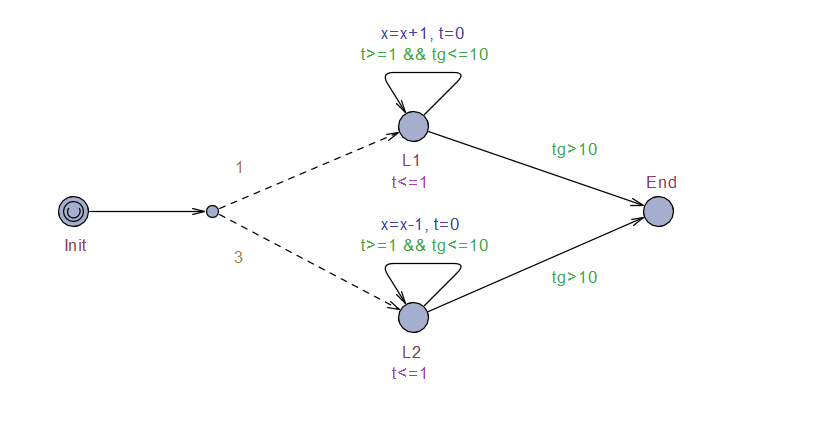
\includegraphics[scale=0.5]{./pictures/uppaal_model_example.png}
	\caption{Uppaal Model}
	\label{uppaal_Model}
\end{figure}

\begin{figure}[h]
	\centering
	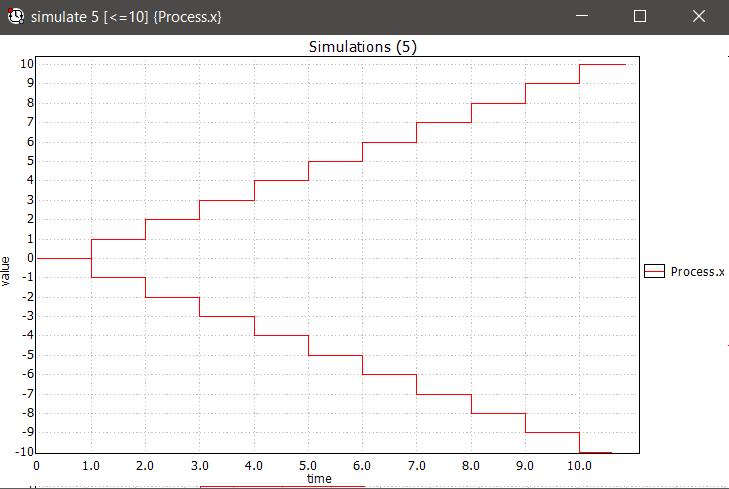
\includegraphics[scale=0.6]{./pictures/uppaal_model_example_simulation.png}
	\caption{Uppaal Simulation Trace Graph}
	\label{uppaal_Simulation_Graph}
\end{figure}

\begin{figure}[h]
	\centering
	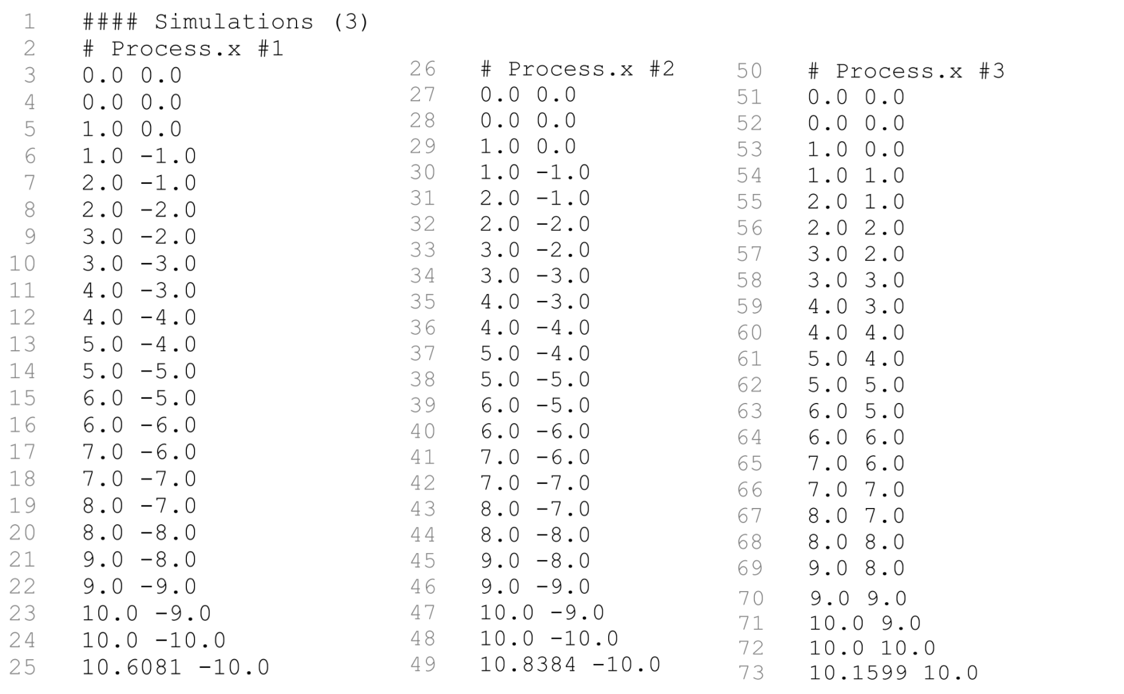
\includegraphics[scale=0.5]{./pictures/simulation_trace.png}
	\caption{Uppaal Simulation Trace Data}
	\label{uppaal_Simulation_Trace}
\end{figure}

\section{Graph Theory}
In the implementation of this project, we represent observations of system simulations as \textit{directed acyclic graphs}, also called \textit{learned models}, by applying variants of techniques like \textit{graph matching} and \textit{graph edit distance} with the incorporation of distance metrics like \textit{Euclidean distance} in an incremental fashion. Therefore we begin by giving the definition of a graph and then an overview of the previous techniques. A more detailed explanation of the mentioned subjects can bee seen in the following two papers of Vincenzo Carletti \cite{graphMatching} and Bengoetxea Endika \cite{theGraphMatchingProblem}. The first paper mainly focuses on graph edit distance and graph theory, while the other on the graph matching problem. Nevertheless, it is important to mention that the graph matching problem is categorized as NP-Complete.

\subsection{Graph Definition}
A graph is a structure $G=(V,E)$ composed of two finite sets: a node set $V$ (or vertices) that represents objects in a domain and an edge set $E \subseteq V \times V$ which represent the relationships among objects. Each edge $e \in E$ is a couple of nodes $e=(u,u')$ where the nodes connected are called \textit{adjacent}. The set $adj(u) = \{ u' \in V | \exists (u,u') \in E \}$ of the nodes adjacent to $u$ is commonly named neighborhood. If the couple $(u,u')$ is ordered, the edge $e$ is said to be directed. A \textit{directed graph} is a graph in which all edges are directed or oriented from one node to another. A directed graph is considered $acyclic$ if the directed graph has a topological ordering, such that for every directed edge $uv$ from node $u$ to node $v$, $u$ comes before $v$ in the ordering.\\ \\ \\ \\
%
Graphs can also bring semantic information by the use of labels and attributes. We take advantage of this properties to map probabilistic timed automata along their components as directed acyclic graphs.
%
\theoremstyle{definition}
\begin{definition}{(Labeled Graph)}
	A labeled graph is a tuple $G= (V,E,\mu, v)$ where
	\begin{itemize}
		\item[--]
		$L$ is a finite alphabet of nodes and edges labels.
		\item[--]
		$\mu: V \rightarrow L$ is a node labeling function. 
		\item[--]
		$v: E \rightarrow L$ is an edge labeling function.  
	\end{itemize} 
\end{definition}

\theoremstyle{definition}
\begin{definition}{(Attributed Graph)}
	Similarly, given that $\mathbb{A}$ is a set of structured information . An attributed graph is a tuple $G= (V,E,\alpha, \gamma)$ where
	\begin{itemize}
		\item[--]
		$\alpha: V \rightarrow \mathbb{A}$ is a node attribute function. 
		\item[--]
		$\gamma: E \rightarrow \mathbb{A}$ is an edge attribute function. 
	\end{itemize} 
\end{definition}


\subsection{Graph Matching}
In pattern recognition, an important problem consists of finding a mapping between the nodes and edges of two graphs, that satisfy a given set of structural constraints. Such problem is commonly known as the \textit{graph matching problem}, whose goal is to find structural correspondence between graphs. 

\subsection{Exact Matching}
\theoremstyle{definition}
\begin{definition}{(Exact graph matching)}
Given two graphs, model graph $G _{M} = (V_ {M}, E_{M})$ and data graph $G _{D} = (V_ {D}, E_{D}),$ with $|V_ {M}| = |V_ {D}|$, the problem is to find a one-to-one mapping $f : V_ {D} \rightarrow V_ {M}$ such that $(u,v) \in E_{D}$ iff $(f(u), f(v)) \in E_{M}$. When such a mapping $f$ exists, $G_D$ is said to be isomorphic to $G_M$. 
\end{definition}

\subsection{Inexact Matching} 
In some real situations the variability of the patterns, the noise in the processes or other causes, may produce deformation in the observed graphs. So two graphs may have similar structures, but with some extra or missing nodes and edges. For these cases, the conditions of exact graph matching are too strict to find out a mapping between two graphs. The most adopted solution is to make the matching process tolerant to deformations by introducing matching costs to penalize structural differences. The closer the structures of two graphs are, the lower is the cost to match them. A well known method to define the matching cost is the \textit{graph edit distance}, which assigns a cost to each operation needed to transform one graph into another one. Please refer to Fig. \ref{graph_edit_distance} for an example of the graph edit distance technique. 
%
\theoremstyle{definition}
\begin{definition}{(Graph edit operations)}
	a graph edit operation is one of the following operations applied on a graph: Node/Edge removal, Node/edge insertion, Node/Edge substitution.
\end{definition}
%
\theoremstyle{definition}
\begin{definition}{(Edit path)}
	an edit path of a graph $G$ is a sequence of elementary operations applied on $G$. It is possible to assign a cost to each simple operation. Among all possible transformations that involve two graphs $G1$ and $G2$, we are interested in the cheapest one, whose cost is the graph edit distance $d(G1,G2)$ between $G1$ and $G2$. 
\end{definition}
%
\begin{figure}[t]
	\centering
	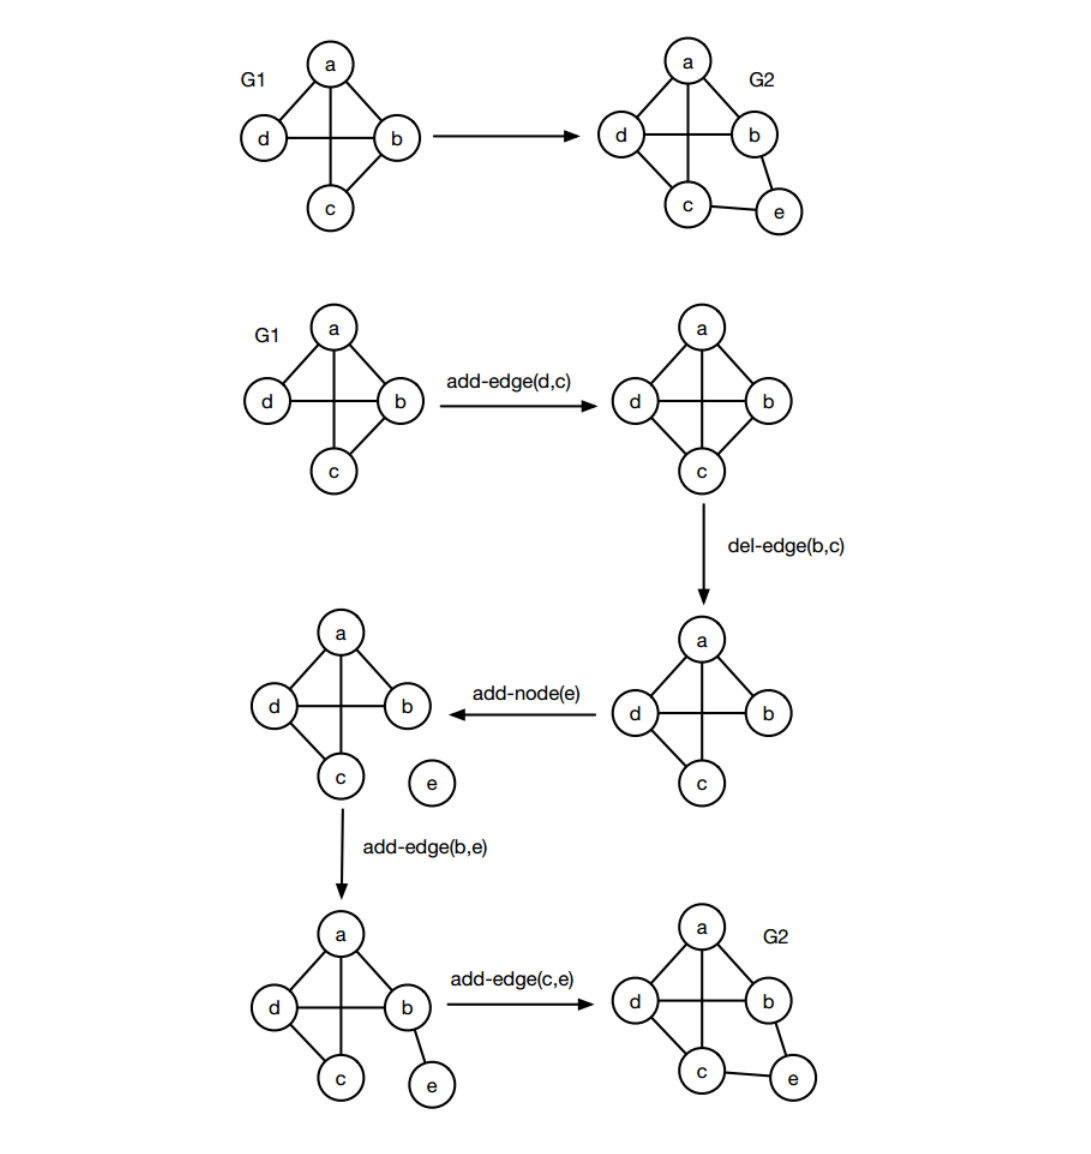
\includegraphics[scale=0.5]{./pictures/graph_edit_distance.png}
	\caption{Graph edit distance example. Illustration taken from \cite{graphMatching}}
	\label{graph_edit_distance}
\end{figure}

\subsection{The Assignment Problem} 
Graph edit distance compares two graphs with \textit{static structures} that do not change over time. We on the other hand, apply a similar approach incrementally and on the fly, as we attempt to match graphs with \textit{dynamic structures} that change over time. Despite this difference, both approaches share another problem, which is the assignment of nodes from one graph to the other. We tackle this issue by mapping the nodes of graphs with the use of the euclidean distance as a mapping function. Further details are given in \Cref{chap:incremental_Learning}
%
\theoremstyle{definition}
\begin{definition}{(Assignment)}
	an assignment is usually represented as a bijective mapping $\varphi: X \rightarrow Y$ between two finite sets $X= \{ x_i \}_i$ and $Y= \{ y_i \}_i$ of size $|X| = |Y| = n$. By assigning the $n$ elements of $X$ to the $n$ elements of $Y$ we get an assignment $\varphi$ corresponding to a permutation $(\varphi(1), \dots, \varphi(n))$, where the first element is assigned to $\varphi(1)$, the second to $\varphi(2)$ and so on.
\end{definition}

\theoremstyle{definition}
\begin{definition}{(Euclidean distance)} \cite{eucledianDistance}
	The euclidean distance or euclidean metric is the ordinary straight-line distance between two points in euclidean space. With this distance, euclidean space becomes a metric space. In Cartesian coordinates, the euclidean distance of between ponint $p=(p_1, p_2, \dots, p_n)$ and point $q=(q_1, q_2, \dots, q_n)$ is given by:
	\begin{equation}
		d(p,q) = d(q,p) = \sqrt{(q_1 - p_1)^2 + (q_2 - p_2)^2 + \dots (q_n - p_n)^2} = \sqrt{\sum_{i=1}^{n} (q_i - p_i)^2}
	\end{equation}
\end{definition}


%\section{Automata Learning}
%Generally explain how learning can be applied or used in timed automata. 
%
%\subsection{Active and Passive}
%General explanation of active and passive learning in timed automata learning. \newpage
 